\clearpage{\pagestyle{empty}\cleardoublepage}
\chapter{Contesto e Stato dell’Arte}

Nella progettazione di applicazioni moderne, i sistemi di gestione dei dati sono fondamentali per garantire efficienza, scalabilità e sicurezza.

Secondo \cite{Elm17}, "i sistemi di gestione dei dati relazionali sono essenziali per strutturare informazioni complesse e garantire accessibilità e coerenza."

Tuttavia, molti database non rispondono a questi requisiti, rendendo necessaria la loro reingegnerizzazione.

Come notato da \cite{Cod70}, "la mancanza di una progettazione documentata può aumentare la difficoltà di manutenzione dei sistemi legacy".

Il presente progetto di tesi affronta queste problematiche, con l'obiettivo di migliorarne l'accesso e l'organizzazione dei dati, integrando funzionalità avanzate come la registrazione, l'autenticazione e il caricamento di dati tramite file.


\section{Struttura dei dati complessa e poco documentata}
Una delle principali problematiche che affliggono i database legacy riguarda la complessità della loro struttura dati, derivata da progettazioni iniziali inadeguate o da una documentazione non aggiornata. La mancanza di una strategia di ottimizzazione nella progettazione porta a database poco flessibili e difficili da manutenere, dove è comune trovare duplicazione di dati, tabelle ridondanti e relazioni mal strutturate. 

Vediamo alcuni degli effetti principali di questa complessità e le possibili soluzioni per rendere la struttura dati più snella e comprensibile.


\begin{itemize}
    \item \textbf{Difficoltà di manutenzione:} La complessità strutturale di un database aumenta esponenzialmente la difficoltà di manutenzione. Ad esempio, modifiche a una singola colonna possono richiedere interventi in molte tabelle interconnesse, con un rischio maggiore di introdurre errori.
    \item \textbf{Problemi di onboarding per nuovi sviluppatori:} La mancanza di documentazione aggiornata limita la comprensione del funzionamento complessivo del database, rallentando i tempi di sviluppo e aumentando il rischio di errori.
    \item \textbf{Duplicazione dei dati:} L’adozione di soluzioni temporanee e la mancanza di normalizzazione possono portare alla duplicazione dei dati, incrementando l’uso di risorse e i rischi di inconsistenza.
\end{itemize}

\subsubsection{Esempio di Struttura Complessa in un E-commerce}
Immaginiamo un database per un sito di e-commerce, originariamente progettato per gestire un numero limitato di prodotti e ordini. Con il tempo, l'azienda ha aggiunto moduli per la gestione di recensioni, promozioni e programmi fedeltà. Tuttavia, tali funzionalità sono state integrate senza una revisione della struttura dati iniziale, portando a una complessità eccessiva. Questo tipo di espansione non pianificata genera tabelle duplicate, ridondanza di dati e query lente a causa dell'elevato numero di join tra tabelle. 

Un processo di reingegnerizzazione potrebbe risolvere questi problemi attraverso la normalizzazione e l’eliminazione delle ridondanze, migliorando significativamente le prestazioni e la manutenibilità del database.


\subsubsection{Soluzioni per Semplificare la Struttura}
La reingegnerizzazione del database comprende tecniche di normalizzazione, eliminazione delle tabelle duplicate e una revisione della documentazione.


\begin{itemize}
    \item \textbf{Normalizzazione:} La normalizzazione consiste nel ridurre la ridondanza dei dati organizzando gli attributi in modo che non vi sia ripetizione di informazioni tra tabelle.

    La normalizzazione, secondo \cite{Sil19}, "è una tecnica fondamentale per migliorare l'integrità e l'efficienza dei database."
    
    Ad esempio, una struttura normalizzata permette di separare le informazioni dei clienti (nome, indirizzo, email) dalle loro transazioni (prodotti acquistati, quantità).
    \item \textbf{Eliminazione delle ridondanze:} Identificare e rimuovere le tabelle duplicate è un passaggio fondamentale. Ad esempio, se due tabelle contengono informazioni molto simili sui clienti, è utile consolidare questi dati in un'unica tabella e creare delle viste che permettano di estrarre le informazioni necessarie senza duplicazione.
    \item \textbf{Documentazione aggiornata:} Una delle soluzioni più semplici ma efficaci è quella di mantenere una documentazione costante della struttura del database. Strumenti come Entity Relationship Diagrams (ERD) o piattaforme come Confluence o GitHub Wiki possono essere utilizzati per tracciare tutte le modifiche.
\end{itemize}

La reingegnerizzazione della struttura non solo rende il database più facile da manutenere, ma riduce anche i rischi legati agli errori umani e migliora l'efficienza generale del sistema.

\subsection{Scalabilità Limitata}
La scalabilità è un aspetto cruciale per i database moderni, in quanto consente al sistema di gestire crescenti volumi di dati e richieste mantenendo buone prestazioni. I database legacy, tuttavia, spesso non supportano una scalabilità ottimale, poiché non sono stati progettati per crescere con facilità. 

Il confronto tra SQL e NoSQL dimostra come "i database NoSQL spesso si adattino meglio a sistemi scalabili" \cite{Sto10}.

Esistono due approcci principali alla scalabilità: la scalabilità verticale e la scalabilità orizzontale.

Come descritto in \cite{Geo11}, "la scelta della strategia di scalabilità dipende spesso dalla natura del carico di lavoro e dall'architettura dell'applicazione."

\subsubsection{Scalabilità verticale}
La scalabilit\'a verticale, o scaling-up, consiste nell'aumentare le risorse hardware di un server per gestire carichi di lavoro crescenti. Tuttavia, questo approccio ha limiti fisici e costi elevati, risultando praticabile solo per una crescita a breve termine. 

\subsubsection{Scalabilità orizzontale}
La scalabilità orizzontale, o scaling-out, distribuisce il carico di lavoro su più server, un metodo comunemente utilizzato nei sistemi distribuiti e nei servizi cloud come AWS e Google Cloud. Questo approccio consente una crescita sostenibile, ma non tutti i database legacy supportano questa architettura.


\subsubsection{Problemi di Scalabilità nei Database Relazionali}
I database relazionali centralizzati come MySQL e PostgreSQL presentano colli di bottiglia quando il numero di utenti simultanei cresce.


\subsubsection{Soluzioni Moderne per la Scalabilità}
Con l’aumento dei dati e delle richieste applicative, la scalabilità è diventata una caratteristica essenziale per i database moderni. Database distribuiti e cloud-native, come Google Cloud Spanner e Amazon Aurora, offrono funzionalità avanzate per la distribuzione geografica e la scalabilità orizzontale, riducendo la latenza e migliorando l’accessibilità globale dei dati. Questi sistemi non solo gestiscono più facilmente grandi volumi di dati, ma supportano anche il ridimensionamento automatico delle risorse.

\paragraph{Caching Distribuito}
Tecnologie come Redis e Memcached migliorano le prestazioni riducendo il carico sui database principali e consentendo l'accesso rapido ai dati più utilizzati. 

"Il caching è essenziale per applicazioni ad alte prestazioni", come sottolineato in \cite{Dea08}.


Questo approccio è particolarmente utile in applicazioni che richiedono risposte in tempo reale.

\subsection{Performance Inefficace}
Le prestazioni di un database sono fondamentali per le applicazioni che lo utilizzano. Una scarsa performance può manifestarsi in tempi di risposta lenti delle query, blocchi nelle transazioni o un uso inefficiente delle risorse hardware. Questo problema è particolarmente presente nei database legacy, dove scelte di progettazione o configurazioni non ottimali ne compromettono l'efficienza.

\subsubsection{Indicizzazione inefficiente}
Uno dei principali problemi delle prestazioni è l'indicizzazione inefficiente o assente. Gli indici accelerano l'accesso ai dati, riducendo il tempo necessario per eseguire le query.

"La gestione degli indici è una pratica cruciale per ottimizzare le prestazioni nei database relazionali" \cite{Elm17}.

Tuttavia, se gli indici non sono ben configurati, le prestazioni del sistema ne risentono notevolmente.

\paragraph{Esempio di Problema}
Supponiamo che una tabella di un e-commerce contenga milioni di record di transazioni. Senza un indice sulla colonna ID cliente, la ricerca delle transazioni di un cliente specifico richiederà la scansione dell'intera tabella, causando ritardi significativi.

\paragraph{Soluzione: Aggiunta di Indici}
Aggiungere indici alle colonne chiave, come gli ID dei clienti o i codici di prodotto, migliora drasticamente le prestazioni delle query. Tuttavia, l'uso eccessivo di indici rallenta le operazioni di scrittura, quindi è importante trovare un compromesso.

\subsubsection{Query subottimali}
Le query mal scritte o subottimali possono avere un impatto devastante sulle prestazioni del database, specialmente quando coinvolgono un numero elevato di join o condizioni non indicizzate. Query SQL che non sono ottimizzate possono causare rallentamenti significativi, poiché il database impiega più tempo per elaborare e restituire i risultati.

\paragraph{Esempio di problema}
Un esempio comune è rappresentato dalle query che coinvolgono molteplici join tra tabelle di grandi dimensioni. Una query che unisce cinque o sei tabelle, senza una progettazione adeguata e senza l'uso di indici, può richiedere un tempo di esecuzione molto lungo. Inoltre, query con funzioni aggregate (come \texttt{COUNT}, \texttt{SUM}, \texttt{AVG}) su tabelle non indicizzate possono ulteriormente peggiorare le prestazioni.

\paragraph{Soluzione: Ottimizzazione delle query}
L'ottimizzazione delle query è un processo che include vari passaggi, come:
\begin{itemize}
    \item \textbf{Uso degli indici:} Come menzionato in precedenza, l'utilizzo di indici sulle colonne giuste può ridurre drasticamente i tempi di esecuzione delle query.
    \item \textbf{Query più semplici:} Ridurre il numero di join e semplificare le condizioni delle query può accelerare il recupero dei dati. Ad esempio, suddividere una query complessa in più query più semplici può spesso produrre risultati migliori.
    \item \textbf{Evitare funzioni sulle colonne:} Funzioni come \texttt{UPPER()}, \texttt{LOWER()} o \texttt{TRIM()} nelle condizioni delle query impediscono l'uso degli indici, poiché il database deve applicare la funzione a ciascun valore prima di eseguire il confronto. È preferibile eseguire la trasformazione dei dati all'interno del codice applicativo, quando possibile.
    \item \textbf{Caching dei risultati:} In alcuni casi, è possibile memorizzare nella cache i risultati di query complesse o frequenti, utilizzando tecnologie come Redis o Memcached. Ciò riduce il carico sul database e velocizza l'accesso ai dati.
\end{itemize}

\subsubsection{Problemi di progettazione delle tabelle}
Un'altra causa di inefficienza delle prestazioni può risiedere nella progettazione stessa delle tabelle. Le tabelle mal progettate, con una struttura dati non ottimizzata, possono portare a problemi di frammentazione dei dati e ad una gestione inefficiente dello spazio di archiviazione.

\paragraph{Esempio di problema}
Un problema comune è la denormalizzazione prematura delle tabelle, che comporta la duplicazione dei dati. Ad esempio, una tabella che memorizza informazioni sugli ordini potrebbe includere campi ridondanti come il nome del cliente o l'indirizzo di spedizione, informazioni che dovrebbero essere memorizzate in una tabella separata. Questa ridondanza non solo occupa spazio di archiviazione extra, ma rende anche più lento il processo di aggiornamento e modifica dei dati.

\paragraph{Soluzione: Normalizzazione e partizionamento}
\begin{itemize}
    \item \textbf{Normalizzazione:} L'applicazione delle regole di normalizzazione può ridurre la duplicazione dei dati e migliorare le prestazioni del database. Le prime tre forme normali (1NF, 2NF e 3NF) sono generalmente sufficienti per la maggior parte delle applicazioni, garantendo che i dati siano suddivisi in tabelle che rappresentano entità uniche e correlate tra loro tramite chiavi esterne.
    \item \textbf{Partizionamento delle tabelle:} Per database molto grandi, è utile implementare il partizionamento delle tabelle. Questo comporta la suddivisione dei dati di una tabella in più parti, o partizioni, che possono essere distribuite su diversi dischi o server. Ad esempio, una tabella di transazioni può essere partizionata in base all'anno della transazione, riducendo così la quantità di dati che deve essere esaminata da ogni query.
\end{itemize}

\subsubsection{Uso inefficiente delle risorse hardware}
Infine, l'uso inefficiente delle risorse hardware, come CPU, memoria e spazio su disco, può ridurre notevolmente le prestazioni del database. Spesso, questo problema si verifica quando non vengono monitorate correttamente le risorse disponibili, oppure quando il sistema non è configurato per distribuire il carico in modo ottimale.

\paragraph{Esempio di problema}
In un sistema che gestisce grandi volumi di dati, la memoria (RAM) svolge un ruolo fondamentale nella gestione della cache del database e nella velocità di accesso ai dati. Se la quantit\`a di RAM disponibile \\è insufficiente, il sistema inizier\`a a utilizzare lo spazio su disco per archiviare temporaneamente i dati (swapping), rallentando drasticamente le prestazioni.

\paragraph{Soluzione: Monitoraggio e tuning}
Il monitoraggio continuo delle risorse hardware, combinato con il tuning del database, può migliorare significativamente le prestazioni. Strumenti come \texttt{Prometheus}, \texttt{Grafana}, e i sistemi di monitoraggio nativi dei database possono essere utilizzati per rilevare i colli di bottiglia e ottimizzare l'allocazione delle risorse.

\subsection{Sicurezza Insufficiente}
La sicurezza dei dati rappresenta una priorità nella progettazione dei database moderni, specialmente alla luce delle attuali minacce informatiche, sempre più complesse e frequenti.

Le linee guida OWASP del 2023 offrono un elenco delle principali vulnerabilità nei sistemi web \cite{OWA23}.

Soluzioni avanzate come i database cloud-native forniscono nuovi strumenti per una gestione scalabile e sicura delle informazioni, con funzionalità integrate di crittografia e accesso controllato.

Le principali sfide di sicurezza nei database legacy includono la protezione dei dati sensibili, la gestione sicura delle credenziali e la prevenzione di accessi non autorizzati. La necessità di un approccio alla sicurezza più strutturato e aggiornato è fondamentale per ridurre i rischi e proteggere le risorse critiche.


Di seguito esaminiamo le principali problematiche di sicurezza nei database tradizionali e le soluzioni pi\'u moderne per affrontarle.

\subsubsection{Protezione dei dati sensibili}
Molti database legacy non implementano misure sufficienti per proteggere i dati sensibili, come informazioni finanziarie, dati personali, o credenziali di accesso. In alcuni casi, queste informazioni vengono memorizzate in chiaro all\'interno del database, esponendole a rischi significativi in caso di accesso non autorizzato.

\paragraph{Esempio di problema}
Un esempio comune è la memorizzazione in chiaro delle password degli utenti. Se un database che contiene password non crittografate viene compromesso, gli aggressori possono facilmente ottenere l'accesso a una vasta quantità di account. Inoltre, in molti casi, lo stesso utente potrebbe utilizzare la stessa password su diversi servizi, aumentando il rischio di attacchi a catena.

\paragraph{Soluzione: Crittografia dei dati}
Una delle soluzioni principali per proteggere i dati sensibili è l'uso della crittografia. 

"La crittografia delle password e dei dati sensibili è una pratica raccomandata per ridurre i rischi di accesso non autorizzato" \cite{Sch15}.

In particolare:
\begin{itemize}
    \item \textbf{Crittografia delle password:} Le password devono essere crittografate utilizzando algoritmi sicuri come \texttt{bcrypt}, \texttt{argon2} o \texttt{PBKDF2}, che includono tecniche di hashing e salting. Questi algoritmi garantiscono che anche se un aggressore ottiene accesso al database, non possa facilmente risalire alla password originale.
    \item \textbf{Crittografia dei dati sensibili:} Oltre alle password, è essenziale crittografare anche altri dati sensibili come i numeri di carte di credito, i dati sanitari o le informazioni di identificazione personale (PII). L'uso di crittografia simmetrica (AES) o asimmetrica (RSA) permette di proteggere i dati sia a riposo (stored data) che in transito (data in transit).
\end{itemize}

\subsubsection{Gestione delle credenziali e autenticazione debole}
Molti sistemi legacy implementano meccanismi di autenticazione che non sono più sicuri rispetto agli standard moderni. Ad esempio, l'uso di credenziali deboli (password semplici o non aggiornate), insieme all'assenza di metodi di autenticazione a più fattori, rende il sistema vulnerabile ad attacchi di forza bruta o a tentativi di accesso non autorizzato.

\paragraph{Esempio di problema}
Un problema comune è l'assenza di policy per la complessità delle password. Molti sistemi permettono agli utenti di creare password semplici (come "123456" o "password"), che possono essere facilmente indovinate o violate attraverso attacchi automatizzati.

\paragraph{Soluzione: Autenticazione sicura e multi-fattore}
Per risolvere questi problemi, le migliori pratiche di sicurezza suggeriscono l'implementazione delle seguenti soluzioni:
\begin{itemize}
    \item \textbf{Autenticazione a due fattori (2FA):} L'uso dell'autenticazione a due fattori aggiunge un livello di protezione supplementare. Oltre alla password, l'utente deve fornire un secondo fattore di autenticazione, come un codice inviato via SMS o generato da un'applicazione di autenticazione (ad esempio, Google Authenticator).
    \item \textbf{OAuth e JWT:} L'adozione di standard come OAuth per la gestione dell'autenticazione basata su token offre un metodo sicuro e scalabile per gestire le sessioni utente. JWT (JSON Web Token) permette di creare token sicuri per l'autenticazione delle sessioni, evitando di memorizzare le credenziali in chiaro o di mantenere sessioni lunghe non necessarie.
    \item \textbf{Policy di password robuste:} Implementare una policy che richieda agli utenti di creare password complesse, aggiornare periodicamente le credenziali e impedire il riutilizzo di vecchie password può ridurre significativamente il rischio di compromissione.
\end{itemize}

\subsubsection{Accesso non autorizzato e SQL Injection}
L'SQL Injection è una delle vulnerabilità più comuni nei database, soprattutto in sistemi legacy che non hanno adottato pratiche di programmazione sicura. Questa tecnica permette a un aggressore di eseguire comandi SQL arbitrari su un database attraverso input non validati, portando a possibili fughe di dati, manipolazioni o eliminazioni di tabelle.

\begin{figure}[h]
    \centering
    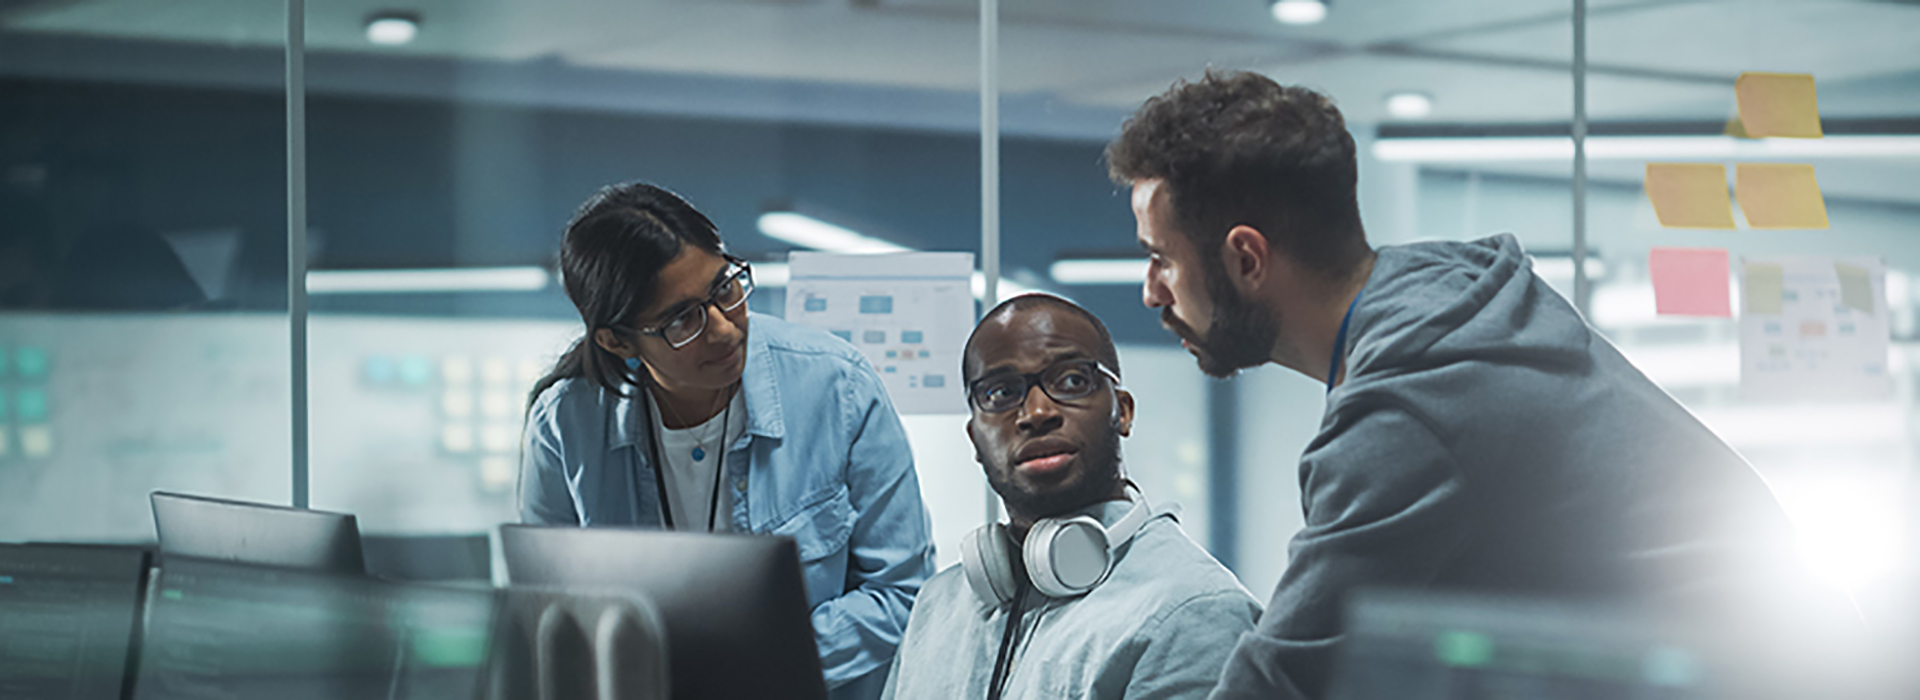
\includegraphics[width=0.8\textwidth]{sources/cybersecurity-team.jpg} % sostituisci con il nome effettivo del file
    \caption{Team di cybersecurity che monitora in tempo reale la sicurezza del database, proteggendo i dati da accessi non autorizzati.}
    \label{fig:team_cybersecurity_monitoraggio}
\end{figure}


\paragraph{Esempio di problema}
Un sito web che accetta input non validati direttamente in una query SQL è vulnerabile a SQL Injection. Ad esempio, un modulo di login che accetta direttamente l'input dell'utente senza adeguata sanitizzazione può permettere a un malintenzionato di inserire un codice malevolo, come:
\[
\texttt{' OR '1'='1'; --}
\]
Questo tipo di attacco può bypassare il normale processo di autenticazione e dare all'aggressore l'accesso al sistema.

\paragraph{Soluzione: Sanitizzazione e query preparate}
La protezione contro SQL Injection si basa su pratiche di programmazione sicura:
\begin{itemize}
    \item \textbf{Query preparate:} L'uso di query preparate o parametriche impedisce l'iniezione di codice SQL non autorizzato. In questo caso, i parametri della query sono trattati come dati e non come comandi SQL.
    \item \textbf{Sanitizzazione degli input:} È fondamentale validare e sanificare ogni input fornito dagli utenti, sia attraverso moduli web, API o altri punti di accesso. Questo garantisce che gli input contengano solo valori attesi, come stringhe alfanumeriche, e non comandi malevoli.
    \item \textbf{Web Application Firewalls (WAF):} Implementare un WAF può aggiungere un ulteriore livello di protezione, monitorando e bloccando automaticamente i tentativi di iniezione SQL o altri attacchi comuni sulle applicazioni web.
\end{itemize}

\subsubsection{Mancanza di controllo degli accessi granulari}
Un altro problema frequente nei database legacy è l'assenza di controlli granulari sugli accessi. Molti sistemi implementano ruoli di accesso rigidi e poco flessibili, che concedono a utenti o applicazioni più permessi di quelli effettivamente necessari per il loro scopo.

\paragraph{Esempio di problema}
In un sistema legacy, è possibile che un utente con ruolo di gestione dei dati abbia accesso completo a tutte le tabelle del database, anche a quelle che non sono pertinenti alle sue mansioni. Questo approccio aumenta il rischio di errore umano o abuso di accesso.

\paragraph{Soluzione: Controllo degli accessi basato su ruoli (RBAC)}
Un moderno approccio alla gestione degli accessi prevede l'implementazione di RBAC (Role-Based Access Control), che limita l'accesso ai dati in base ai ruoli degli utenti. In RBAC, a ogni utente viene assegnato un ruolo specifico con un set limitato di privilegi, garantendo che possa accedere solo alle risorse necessarie per svolgere il proprio lavoro.
\begin{itemize}
    \item \textbf{Principio del minimo privilegio:} Un sistema ben progettato dovrebbe implementare il principio del minimo privilegio, dove gli utenti e le applicazioni possono accedere solo alle risorse minime necessarie per eseguire le proprie operazioni.
    \item \textbf{Monitoraggio e auditing:} Oltre ai controlli di accesso, è importante implementare un sistema di auditing che monitori tutte le attività nel database, generando log dettagliati su chi accede a quali dati e quando. Ciò permette di identificare immediatamente eventuali comportamenti sospetti.
\end{itemize}

\subsubsection{Backup e ripristino dei dati}
Infine, molti database legacy non dispongono di adeguati sistemi di backup e ripristino, rendendo difficile il recupero dei dati in caso di attacco o malfunzionamento. La perdita o compromissione dei dati, in assenza di backup frequenti e sicuri, può avere un impatto devastante.

\paragraph{Esempio di problema}
Un attacco ransomware potrebbe crittografare i dati del database e richiedere un riscatto per il loro ripristino. Senza un sistema di backup sicuro, l'azienda potrebbe perdere definitivamente l'accesso ai dati critici.

\paragraph{Soluzione: Backup regolari e sicuri}
Le migliori pratiche includono:
\begin{itemize}
    \item \textbf{Backup frequenti e automatizzati:} Implementare un sistema di backup regolare, preferibilmente automatizzato, che memorizzi copie aggiornate del database su server separati e sicuri.
    \item \textbf{Test periodici di ripristino:} È importante non solo creare backup, ma anche testare regolarmente il processo di ripristino per assicurarsi che i dati possano essere recuperati rapidamente e senza errori.
    \item \textbf{Crittografia dei backup:} I backup dovrebbero essere crittografati per impedire che informazioni sensibili vengano compromesse anche se i backup stessi vengono rubati o violati.
\end{itemize}
\section{Stato dell’arte nella reingegnerizzazione dei database}
Negli ultimi anni, la reingegnerizzazione dei database ha assunto un'importanza crescente nel campo dell'informatica, spinta dalla necessità di migliorare le prestazioni, la sicurezza e la scalabilità dei sistemi di gestione dei dati. La complessità dei sistemi moderni, l'aumento esponenziale del volume dei dati e le crescenti aspettative degli utenti richiedono l'adozione di tecniche avanzate per gestire, ottimizzare e mantenere i database.

In questa sezione esaminiamo le principali tecnologie e metodologie che attualmente definiscono lo stato dell'arte nella reingegnerizzazione dei database, inclusi ORM, migrazioni di database, database distribuiti.

\subsection{Object-Relational Mapping (ORM)}
L'Object-Relational Mapping (ORM) è una tecnica che consente di mappare le tabelle di un database relazionale agli oggetti nei linguaggi di programmazione orientati agli oggetti. Gli ORM sono strumenti essenziali nel modernizzare la gestione dei database, poiché facilitano la comunicazione tra l'applicazione e il database, riducendo la necessità di scrivere query SQL complesse e rendendo il codice più modulare e manutenibile.

\subsubsection{Come funziona l'ORM}
Gli ORM, come \textbf{Hibernate}, \textbf{Doctrine} e \textbf{Entity Framework}, permettono agli sviluppatori di manipolare i dati del database attraverso oggetti di alto livello senza dover scrivere direttamente il codice SQL. L'ORM genera automaticamente le query SQL necessarie in base alle operazioni eseguite sugli oggetti dell'applicazione. Ad esempio, in un'applicazione e-commerce, una classe "Prodotto" può essere mappata a una tabella "prodotti" nel database. Gli sviluppatori possono quindi lavorare con l'oggetto "Prodotto" nel loro codice, lasciando all'ORM il compito di tradurre le operazioni sugli oggetti in query SQL.

\subsubsection{Vantaggi e limitazioni}
\begin{itemize}
    \item \textbf{Vantaggi:}
    \begin{itemize}
        \item \textit{Astrazione del livello di persistenza}: Gli ORM consentono agli sviluppatori di concentrarsi sulla logica dell'applicazione, senza doversi preoccupare dei dettagli di implementazione delle query SQL.
        \item \textit{Manutenzione semplificata}: Poiché gli ORM separano la logica di business dalla gestione dei dati, il codice diventa più facile da mantenere e aggiornare. Le modifiche alla struttura del database possono essere implementate senza dover riscrivere il codice SQL.
        \item \textit{Riduzione degli errori}: Gli ORM riducono la probabilità di errori umani, come la scrittura di query SQL mal formate o vulnerabili a SQL injection, poiché le query sono generate automaticamente.
    \end{itemize}
    \item \textbf{Limitazioni:}
    \begin{itemize}
        \item \textit{Prestazioni inferiori}: Gli ORM, se non configurati correttamente, possono introdurre un overhead aggiuntivo, rallentando le prestazioni delle applicazioni che devono eseguire un gran numero di operazioni su database molto grandi.
        \item \textit{Query complesse}: Sebbene gli ORM siano molto utili per le operazioni CRUD (Create, Read, Update, Delete), la loro efficacia diminuisce con query più complesse che richiedono ottimizzazioni avanzate o operazioni non standard sui dati.
    \end{itemize}
\end{itemize}

\subsubsection{Strumenti ORM più utilizzati}
Alcuni degli ORM più utilizzati nel settore includono:
\begin{itemize}
    \item \textbf{Hibernate} (Java): Un framework ORM per Java che offre numerose funzionalità avanzate per la gestione dei dati e delle relazioni tra le entità del database.
    \item \textbf{Doctrine} (PHP): Un ORM per PHP che supporta diverse strategie di mapping e include un sistema di migrazioni per mantenere il database allineato con le modifiche apportate al modello di dati.
    \item \textbf{Entity Framework} (C\#/.NET): Lo strumento ORM principale per il framework .NET, che consente di eseguire query LINQ per accedere ai dati tramite oggetti.
\end{itemize}

\subsection{Migrazioni di database}
Le migrazioni di database sono un metodo che permette di applicare modifiche incrementali alla struttura di un database in modo controllato e sicuro. Le migrazioni risolvono uno dei problemi principali nella gestione dei database: come aggiornare la struttura dati senza compromettere i dati esistenti o causare downtime.

\subsubsection{Come funzionano le migrazioni di database}
Con le migrazioni di database, ogni modifica alla struttura del database, come l'aggiunta di una colonna o la modifica di un indice, viene codificata in uno script che può essere eseguito in modo incrementale. Questo approccio consente di mantenere una cronologia delle modifiche, semplificando la gestione delle versioni del database e garantendo che il database di produzione e quelli di sviluppo siano sempre sincronizzati.

Ad esempio, se si vuole aggiungere una nuova colonna "email" alla tabella "utenti", si può scrivere una migrazione che aggiunge la colonna e aggiorna tutti i record esistenti. Se successivamente è necessario rimuovere o modificare questa colonna, un'altra migrazione può essere applicata senza alterare i dati in modo manuale o pericoloso.

\subsubsection{Strumenti per le migrazioni}
Alcuni degli strumenti più popolari per le migrazioni di database includono:
\begin{itemize}
    \item \textbf{Flyway}: Uno degli strumenti di migrazione più popolari, supporta vari tipi di database, come PostgreSQL, MySQL e Oracle. Flyway gestisce le migrazioni attraverso file SQL o script Java.
    \item \textbf{Liquibase}: Uno strumento open-source che consente di eseguire migrazioni di database attraverso script XML, YAML, JSON o SQL. Liquibase offre anche funzionalità di rollback che permettono di annullare facilmente una modifica al database.
\end{itemize}

\subsubsection{Vantaggi delle migrazioni di database}
\begin{itemize}
    \item \textit{Controllo delle versioni}: Le migrazioni permettono di mantenere un registro dettagliato di tutte le modifiche al database, garantendo che l'intero team possa lavorare con la stessa versione della struttura dati.
    \item \textit{Aggiornamenti incrementali}: Ogni modifica è applicata in modo incrementale, riducendo il rischio di errori e permettendo il rollback in caso di problemi.
    \item \textit{Semplicità di implementazione}: Gli strumenti di migrazione sono semplici da integrare nei processi di sviluppo esistenti e possono essere eseguiti automaticamente durante il deploy di una nuova versione dell'applicazione.
\end{itemize}

\subsection{Database distribuiti e cloud-native}
L'evoluzione dei database distribuiti e dei sistemi cloud-native ha cambiato profondamente il modo in cui i database vengono progettati e gestiti. I database distribuiti sono progettati per essere eseguiti su più nodi o server, garantendo un'alta disponibilità e una scalabilità orizzontale, mentre i database cloud-native sono pensati per sfruttare al massimo le infrastrutture cloud.

\subsubsection{Database distribuiti}
I database distribuiti come \textbf{Apache Cassandra}, \textbf{Google Cloud Spanner} e \textbf{CockroachDB} consentono di distribuire i dati su più server o regioni geografiche, garantendo la tolleranza ai guasti e una scalabilità pressoché illimitata. Questi sistemi utilizzano algoritmi di consenso distribuiti, come il \textbf{Paxos} o il \textbf{Raft}, per garantire la coerenza dei dati su tutti i nodi.

\paragraph{Vantaggi dei database distribuiti}
\begin{itemize}
    \item \textit{Alta disponibilità}: La distribuzione dei dati su più nodi garantisce che il sistema rimanga disponibile anche in caso di guasto di uno o più nodi.
    \item \textit{Scalabilità orizzontale}: A differenza dei database relazionali tradizionali, che si basano principalmente sulla scalabilità verticale, i database distribuiti possono scalare orizzontalmente aggiungendo nuovi nodi al cluster.
    \item \textit{Bassa latenza globale}: I database distribuiti possono ridurre la latenza per gli utenti geograficamente distanti, replicando i dati in più regioni e rispondendo alle query dal nodo più vicino.
\end{itemize}

\begin{figure}[h]
    \centering
    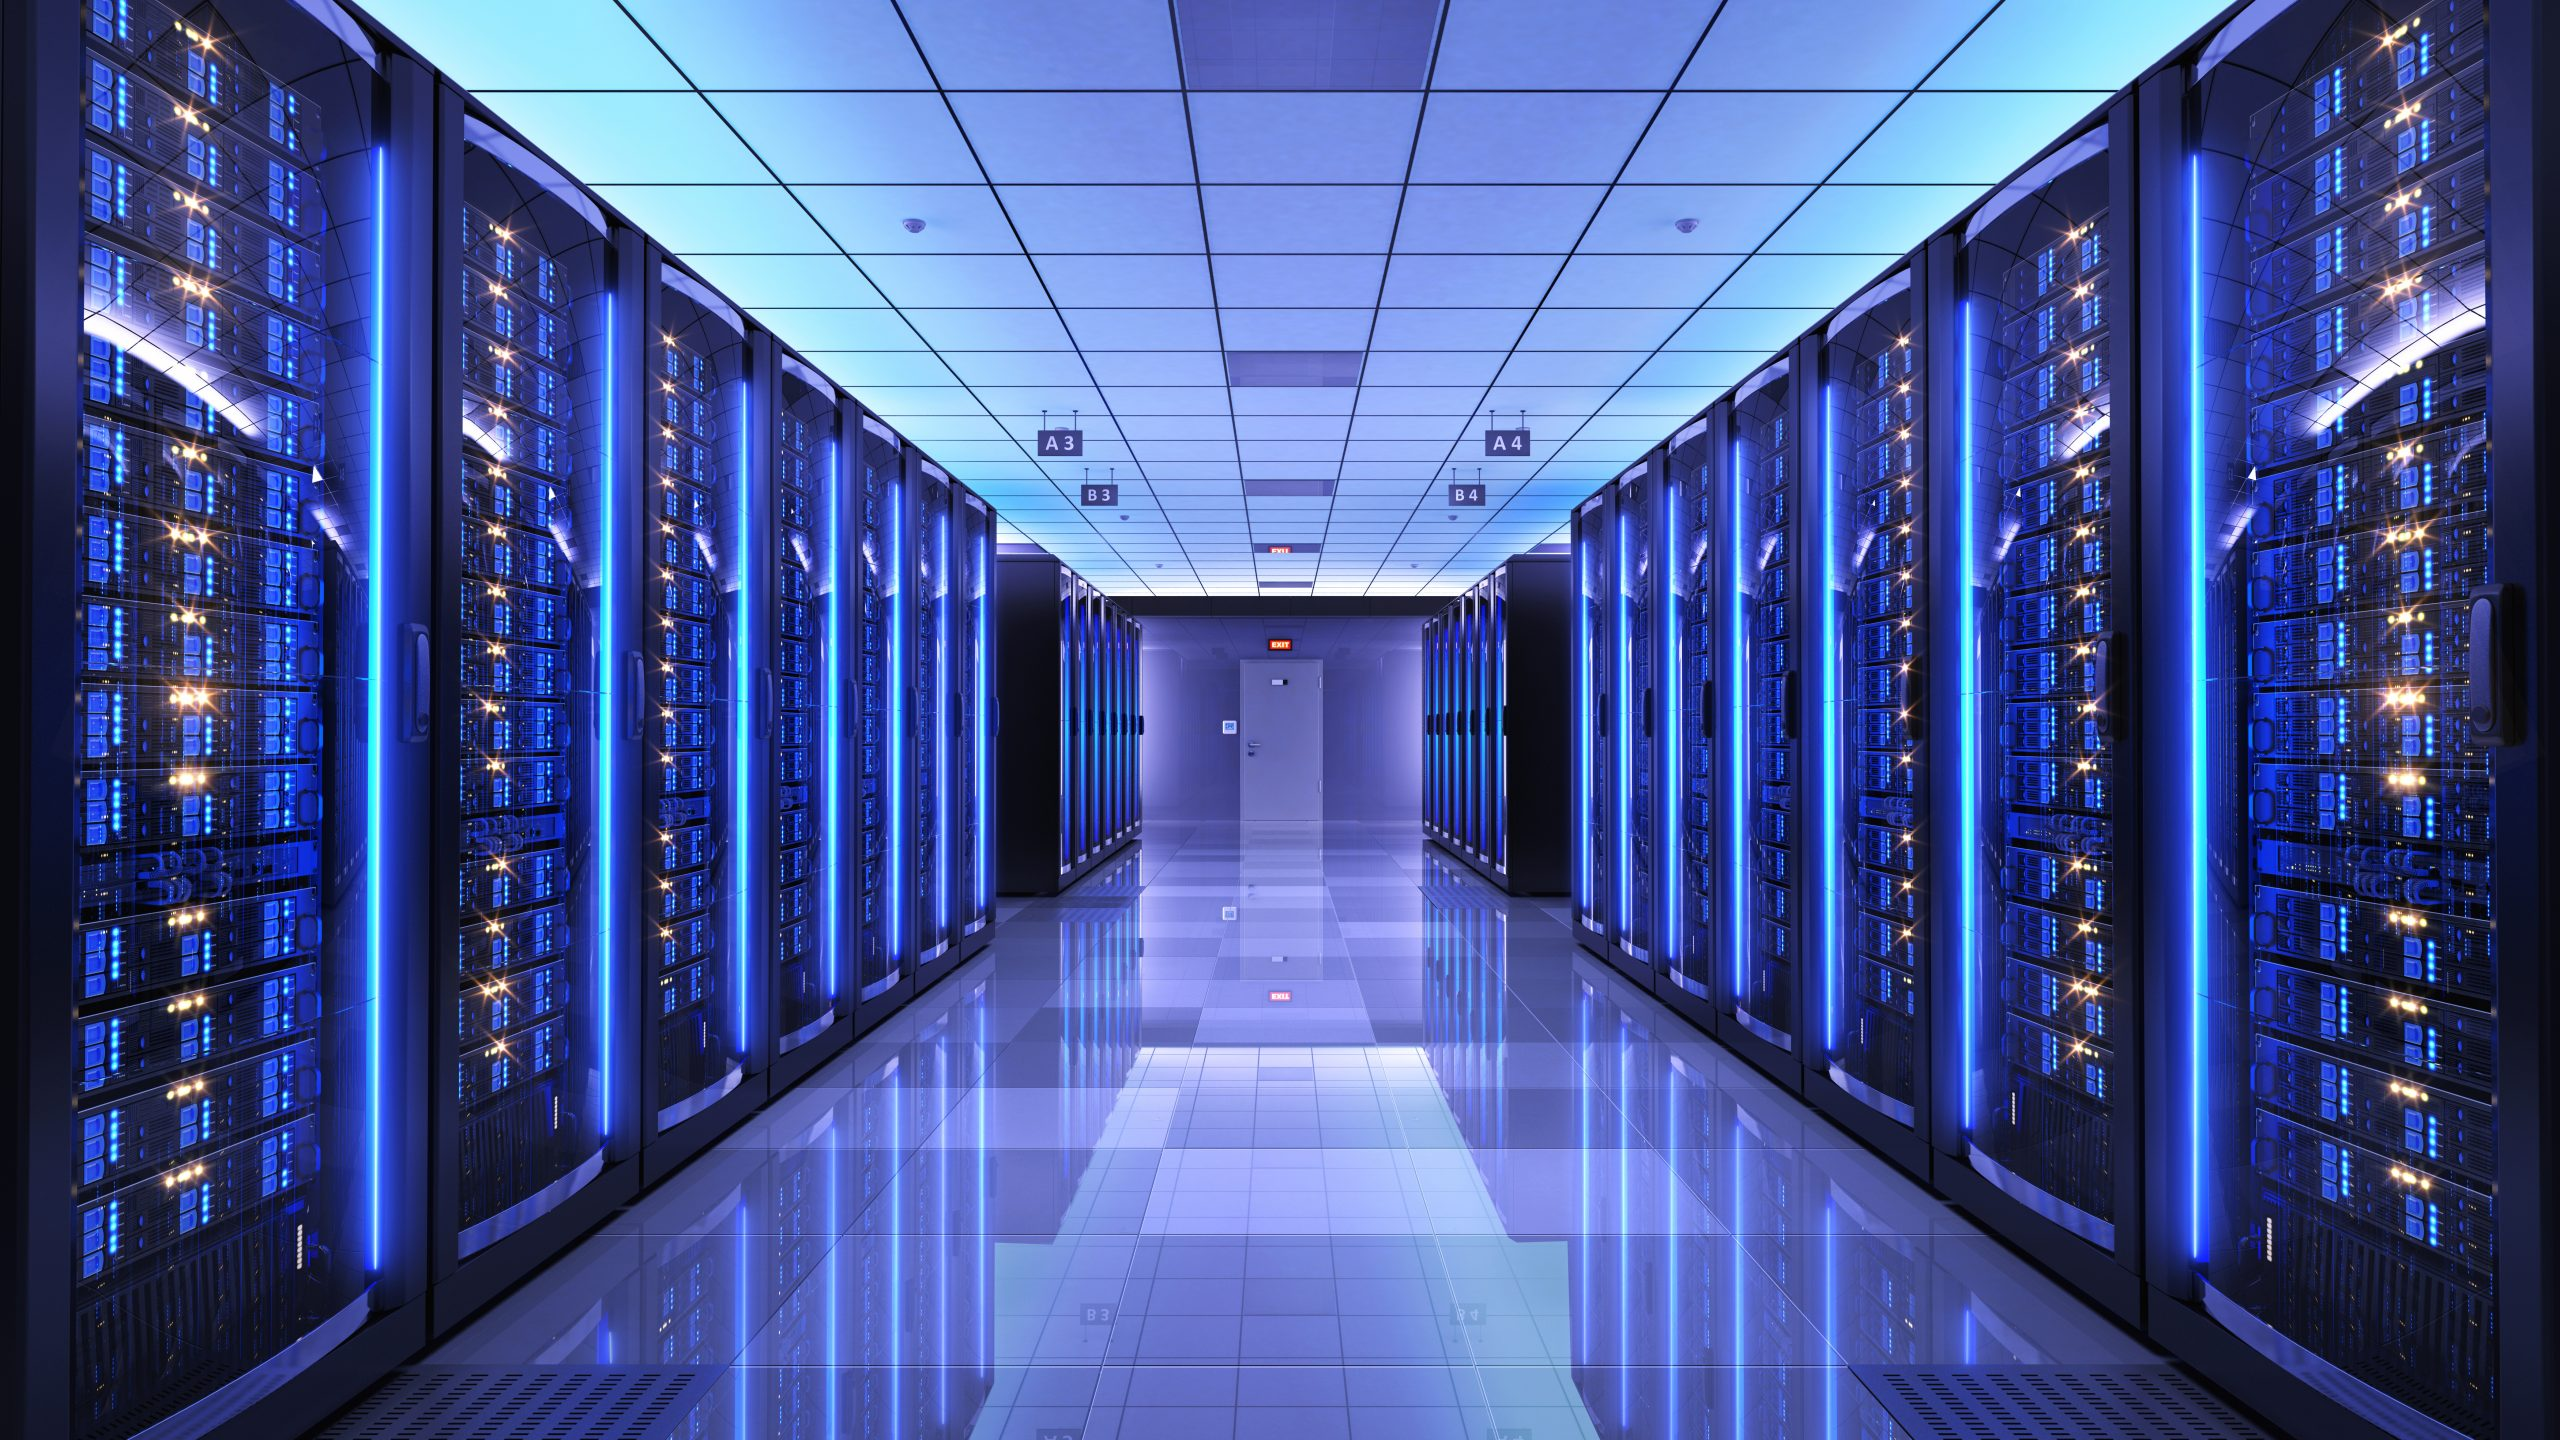
\includegraphics[width=0.8\textwidth]{sources/data-center-scaled.jpeg}
    \caption{Data center moderno che ospita le infrastrutture di database cloud-native.}
    \label{fig:datacenter_cloud}
\end{figure}

\subsubsection{Database cloud-native}
Con l'avvento delle piattaforme cloud, molti database moderni sono stati progettati per sfruttare le caratteristiche uniche del cloud, come l'auto-scaling, il provisioning dinamico delle risorse e il supporto per microservizi. Servizi come \textbf{Amazon RDS}, \textbf{Azure SQL Database} e \textbf{Google Cloud SQL} offrono database relazionali che possono essere facilmente scalati in base al carico e gestiti senza l'intervento manuale del team IT.

\paragraph{Vantaggi dei database cloud-native}
\begin{itemize}
    \item \textit{Gestione semplificata}: I database cloud-native eliminano la necessità di gestire l'infrastruttura fisica, permettendo ai team di sviluppo di concentrarsi esclusivamente sull'ottimizzazione delle query e delle applicazioni.
    \item \textit{Auto-scaling}: Questi database possono scalare automaticamente in base alla domanda, allocando o deallocando risorse in modo dinamico.
    \item \textit{Resilienza incorporata}: I database cloud-native sono progettati per tollerare guasti hardware, garantendo l'alta disponibilità e la continuità operativa.
\end{itemize}

\paragraph{Migrazione verso Database Cloud-Native}
Un esempio significativo è rappresentato dall'adozione di Amazon Aurora da parte di diverse aziende, che hanno scelto di migrare le loro infrastrutture legacy verso soluzioni cloud-native. Questa migrazione ha permesso di ottenere scalabilità, riduzione della latenza e maggiore sicurezza, eliminando la necessità di gestire hardware dedicato e migliorando al contempo la resilienza e la capacità di gestire picchi di traffico.


\section*{Conclusioni}
In questo capitolo, abbiamo esplorato alcune delle principali problematiche che affliggono i database legacy, inclusa la complessità della struttura dati, i limiti di scalabilità e le inefficienze nelle prestazioni. La reingegnerizzazione di un database si propone di risolvere questi problemi, migliorando la manutenibilità, l'efficienza e la sicurezza.

Nel prossimo capitolo, ci concentreremo sulle tecnologie, i linguaggi e i framework utilizzati per la reingegnerizzazione di un database, illustrando le caratteristiche dei sistemi ORM, le strategie di migrazione e le tecniche avanzate di sicurezza.



%\begin{figure}[h]                       %crea l'ambiente figura; [h] sta
                                        %   per here, cioè la figura va qui
%\begin{center}                          %centra nel mezzo della pagina
                                        %   la figura
%\includegraphics[width=5cm]{figura.eps}%inserisce una figura larga 5cm
                                        %se si vuole usare va scommentata
%
%%%%%%%%%%%%%%%%%%%%%%%%%%%%%%%%%%%%%%%%%inserisce la legenda ed etichetta
                                        %   la figura con \label{fig:prima}
%\caption[legenda elenco figure]{legenda sotto la figura}\label{fig:prima}
%\end{center}
%\end{figure}

